\section{Domain Expert Feedback}
\label{sec:feedback}
In this section, we share the invaluable feedback collected from the modelers. 
Meeting \#6 and \#7 were held prior to the conclusion of our development, serving as an iterative process of refinement aimed at validating and improving our visual designs while ensuring their relevance and utility to domain experts.
Meeting \#8 was held after the conclusion of our development, functioning as a means to gather feedback on our work and to identify potential future work.
Here, we present some of the original quotes collected from the domain experts during these meetings.
% \begin{figure}[tb!]
%     \centering
%     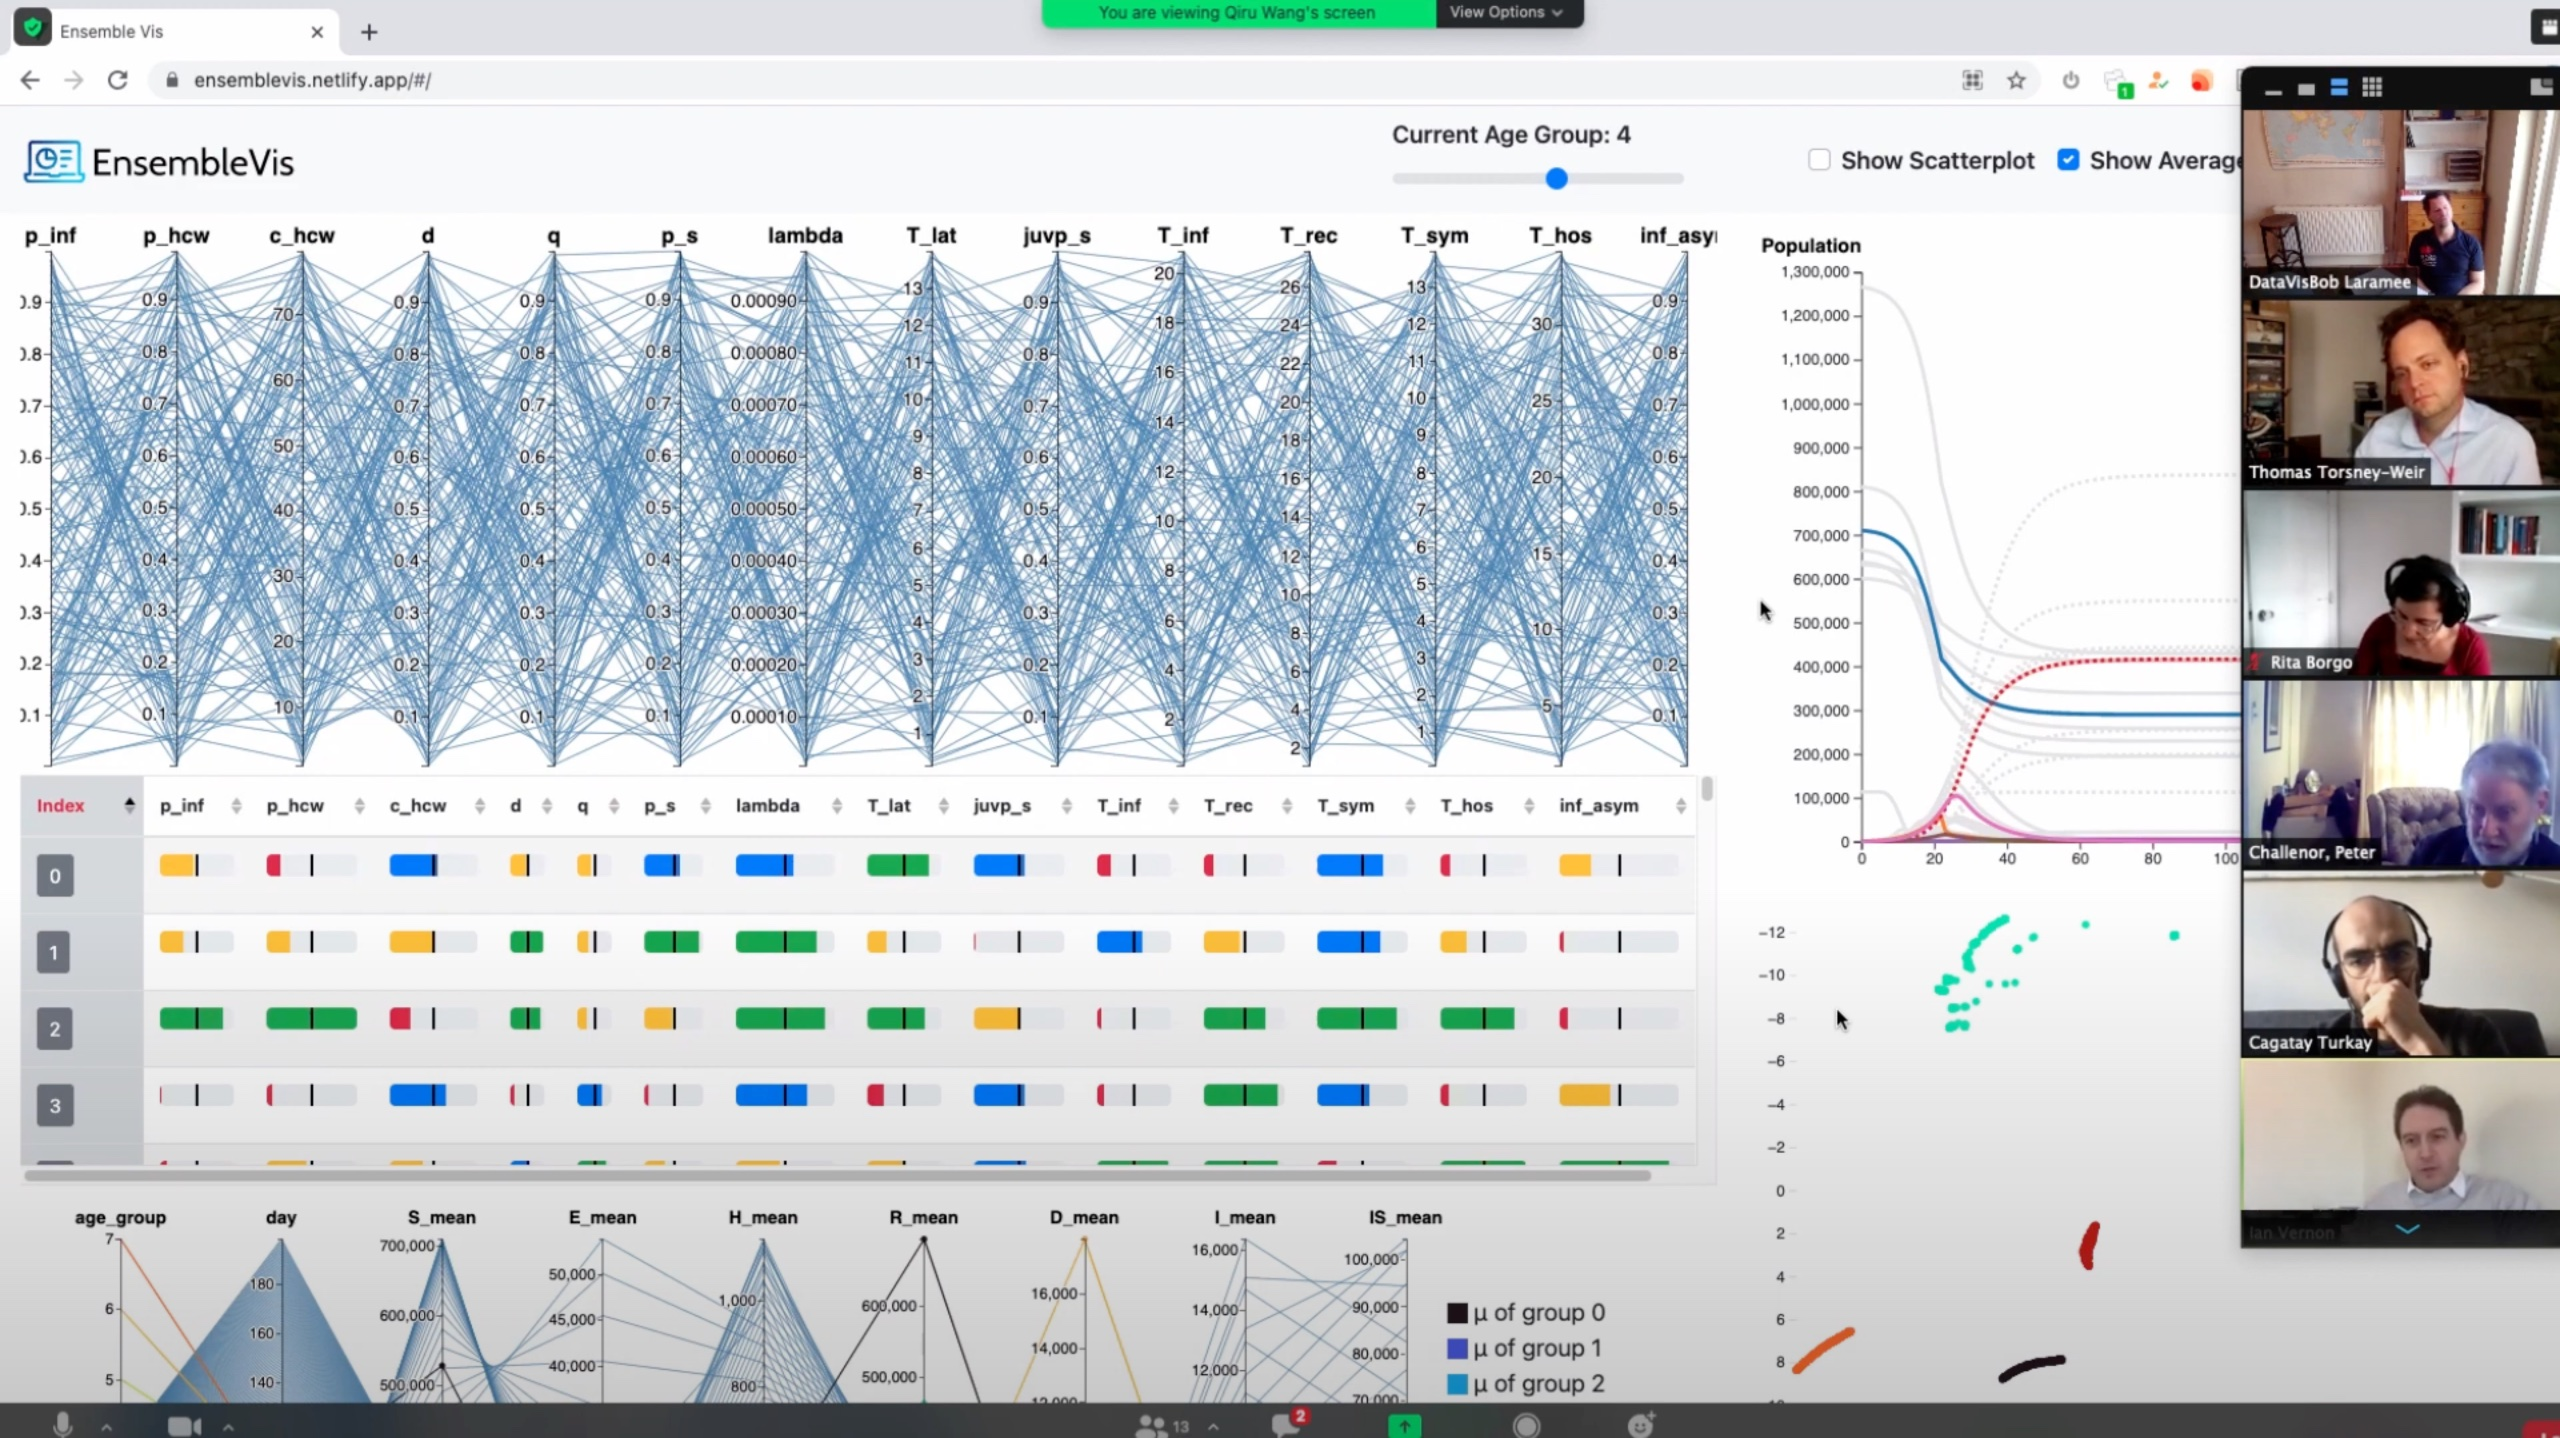
\includegraphics[width=\linewidth]{feedback2.jpeg}
%     \caption{A virtual meeting including six SCRC modelers and five RAMPVis researchers was held on 25 Mar 2021.
%     }
%     \label{fig:feedback2}

% \end{figure}

\bobgraph{Domain Expert \#1 - Professor in Statistics, Durham University}
% Ian Vernon

During our live demonstration, the domain expert appreciated the interactions provided by the visual designs in depicting the relative importance of different input parameters on the model's predictions.
\textit{``The visualizations are able to show how important a particular input is for a particular output.''
    }

In addition, the ability to present the link between the input and output parameters visually.
\textit{``The real interesting game here is the connection techniques to understand the relations between the input and output.''
}

The linked visual designs also potentially enable the domain expert to identify ineffective parameter combinations.
\textit{``The different configurations is the sort of history of calibration and by looking at those visualizations you can start saying certain combinations may not be useful.''
}

Furthermore, the domain expert also expressed interest in the potential of our visual designs to aid in the identification of model discrepancy, when the observational data becomes available.
\textit{``The visualization would be helpful for us to identify model discrepancy when we eventually plot the observational data.''
}

\bobgraph{Domain Expert \#2 - Professor in Statistics, the University of Exeter}
% Peter Challenor

The domain expert was pleased by the visual designs' ability to provide the potential to filter redundant input parameter configurations, enabling users to concentrate on the most influential configurations.
\textit{``For particular input configurations after filtering, the visualization shows some of the input parameters can be ignored, which reduces the dimensionality of the problem, and we can focus on the important parameters.''
}

\bobgraph{Domain Expert \#3 - Assistant Professor in Statistics, the University of Glasgow}
% Ben Swallow
The domain expert praised the visual designs' ability to provide a clear overview of the input parameters and their distributions. This enables them to quickly identify possibility adjustments they can make to their input parameters, as well as to identify the most influential parameters.
\textit{
``The table view is really useful in showing how close those input parameters are to the threshold, which is very useful for us to understand the affordability.''
}

The domain expert also noted that some overlapping distributions can be ruled out quickly via the interactivity provided by our visual designs, this enables them to eliminate unnecessary complexities and increase the overall efficiency of their model.
\textit{
``It's fairly obvious that some of the parameters can be ruled out quite quickly, including some overlapping distributions.''
}

An avenue for future work, as unanimously identified by all three domain experts, involves integrating new visual designs to effectively render and compare observational data against model predictions.
